\documentclass[11pt]{article}

\usepackage[margin=2.4cm]{geometry}
\usepackage{amsmath,amssymb}
\usepackage{graphicx}
\usepackage{booktabs}
\usepackage{hyperref}
\usepackage{microtype}
\usepackage{caption}
\usepackage{xcolor}
\usepackage{listings}
\usepackage{multirow}

\title{\textbf{Topological early-warning detection of a photoinduced structural\\
phase transition: persistent-homology signals validated on IBM quantum hardware}}
\author{Jonathan Evina$^{1,2}$ and JOHNKING0$^{2}$\\
\small $^{1}$ RATISS Labs, Yaound\'e, Cameroon\\
\small $^{2}$ RATISS independent research group\\
\small \texttt{ORCID 0009-0000-4092-5313}}
\date{August 2026}

\begin{document}
\maketitle

\begin{abstract}
Photoinduced structural reorganisation of crystals---charge-density-wave
reconfigurations, light-induced hidden states, photo-controlled
superconducting or topological phases---is detected \emph{a posteriori} by
classical order parameters. Here we ask whether a topological signal computed
from the quantum-state correlation matrix can flag the transition
\emph{before} conventional markers, and we test the answer end-to-end on
real quantum hardware. On the exactly solvable Su--Schrieffer--Heeger (SSH)
chain with a time-driven dimerisation ramp $\delta(t)$, the
persistent-homology lifetime $P_{\mathrm{sig}}$ of the correlation matrix
$|C_{ij}| = |\langle c_i^\dagger c_j\rangle|$ acts as a binary detector of
the topological phase, while the edge--edge correlation $|C_{0,N-1}|$
crosses threshold $3.6$ time units \emph{before} the Hamiltonian reaches
$\delta=0$. Under round-trip ramps the dynamical hysteresis area grows as a
power law $A \propto v^{1.05}$ over 1.5 decades of ramp velocities,
consistent with a Kibble--Zurek-type picture. Against Lindblad dephasing,
the signal survives to $\gamma = 0.05$ at $1/2$ purity. On IBM quantum
hardware (\texttt{ibm\_marrakesh}, $156$ qubits) the raw $P_{\mathrm{sig}}$
contrast \emph{inverts} under decoherence; we show that a coupled score
$S = P_{\mathrm{sig}}(>\!\tau) + |C_{0,N-1}| - 0.1\,H_{C}$ restores a
positive contrast, validated \emph{in situ} on \texttt{ibm\_fez}:
topological $+0.162$ vs trivial $-0.175$ at $N=4$ (contrast $0.337$), and
topological $-0.184$ vs trivial $-0.229$ at $N=8$ (contrast $0.045$). All
code, data and raw hardware job records are public: every number herein is
reproducible from the repository. The method is directly transferable to
transition-metal dichalcogenides (e.g.\ 1T-TaS$_2$) and to any driven
lattice with accessible correlation measurements.
\end{abstract}

\noindent\textbf{Keywords:} persistent homology; early-warning signal;
photoinduced phase transition; SSH model; Kibble--Zurek scaling; IBM Quantum
hardware; topological data analysis; charge density waves.

\section{Introduction}

When a femtosecond laser pulse hits a transition-metal crystal, the lattice
can reorganise into metastable phases: 1T-TaS$_2$ exhibits a hidden charge
density wave (CDW) state \cite{Stojchevska2014,Vaskivskyi2016}, and related
light-driven control of superconducting or topological orders is an active
front \cite{Yoshida2014}. The reorganisation involves domain-wall braiding
and defect dynamics that classical order parameters detect only once the
transition \emph{has occurred}. A predictive, early-warning marker computed
from the evolving quantum state would change experimental practice: it
would let experimentalists anticipate the switch before the lattice locks
in.

Topological data analysis (TDA), in particular persistent homology
\cite{Edelsbrunner,Carlsson}, has recently been shown to detect phase
transitions without labelling them in advance \cite{Tran2021}. The keyword
here is not innocuous: ``topological'' refers both to the TDA machinery and
to the topological phase of the material itself, so there is a double
reason to expect the method to bite on exactly these systems.

In this work we make three contributions.

\begin{enumerate}
\item \textbf{A topological early-warning signal.} On the SSH chain (the
minimal exactly-solvable model of a topological crystal), the edge--edge
correlation $|C_{0,N-1}|$ of the evolving state crosses threshold
time units before the Hamiltonian's transition time $t_c$ where $\delta(t_c)=0$.
The persistent-homology lifetime $P_{\mathrm{sig}}$ of the correlation
matrix acts as a phase-confirmer, and the edge correlation as a
phase-precursor.
\item \textbf{Dynamical hysteresis with a scaling law.} Under round-trip
ramps, the hysteresis loop area obeys $A \propto v^{1.05}$ over 1.5 decades
of velocities, a Kibble--Zurek-type signature of critical slowing down
\cite{Kibble1976,Zurek1985,Dziarmaga2005}.
\item \textbf{End-to-end validation on real quantum hardware.} We show the
raw $P_{\mathrm{sig}}$ contrast \emph{inverts} on IBM hardware, and a
coupled robust score restores a positive contrast on \texttt{ibm\_fez} at
$N=4$ (contrast $0.337$) and $N=8$ (contrast $0.045$), with all job records
public. To our knowledge this is the first TDA-based early-warning marker
measured on quantum processing unit (QPU) hardware.
\end{enumerate}

The remainder of this paper presents the model and methods
(\S\ref{sec:model}), results (\S\ref{sec:results}), an honest discussion of
limitations (\S\ref{sec:limits}), and a conclusion
(\S\ref{sec:conclusion}). All data and code are in the public repository
\cite{repo}.

\section{Model and methods}
\label{sec:model}

\subsection{The driven SSH chain}

We study the Su--Schrieffer--Heeger (SSH) chain \cite{SSH1979,SSH1980} with
open boundaries, $N$ sites and half-filling:
\begin{equation}
H(t) = \sum_{i} \Big[ t_1\,c_i^\dagger c_{i+1} \Big|_{i\text{ odd}} +
t_2\,c_i^\dagger c_{i+1} \Big|_{i\text{ even}} + \mathrm{h.c.}\Big],\quad
t_{1,2} = 1 \pm \delta(t),
\label{eq:ssh}
\end{equation}
where a linear ramp $\delta(t)$ from $+0.4$ to $-0.4$ emulates a light-driven
structural distortion through the exact topological transition at $\delta=0$
\cite{Zak1989}. The winding number $w(\delta)$ changes from $0$ to $1$ and
the edge states appear in the $\delta<0$ phase; this analytic ground truth
makes every marker falsifiable.

\subsection{Correlation matrix and persistence}

At half filling the occupied orbitals define the projector
$C_{ij} = \langle c_i^\dagger c_j\rangle$. We feed the Euclidean distances
between the rows of $|C|$ into the Vietoris--Rips filtration (GF(2)
coefficients, simplices up to triangles) and take
\begin{equation}
P_{\mathrm{sig}} = \max\{\text{finite } H_1 \text{ lifetimes}\},
\label{eq:psig}
\end{equation}
an implementation recast from the auditable RATISS engine \cite{repo}.

The real-time dynamics $i\partial_t\psi_t = H(t)\psi_t$ is propagated by
RK4; the ``adiabatic reference'' recomputes the instantaneous ground state
at each time and is used to discriminate intrinsic dynamical effects from
integration artefacts.

\subsection{Robust coupled score}

QPU decoherence destroys the raw $P_{\mathrm{sig}}$ contrast
(\S\ref{sec:qpu}). We therefore vote three markers:
\begin{equation}
S = \underbrace{P_{\mathrm{sig}}(>\!\tau)}_{\text{persistence above
threshold }\tau=0.05} + \underbrace{|C_{0,N-1}|}_{\text{edge correlation}} -
0.1 \cdot \underbrace{H_{C}}_{\text{correlation entropy}},
\label{eq:score}
\end{equation}
where $H_{C} = -\sum_{ij}|C_{ij}|\log|C_{ij}|/\sum_{ij}|C_{ij}|$ is
subtracted as disorder. The contrast is $\Delta S = S_{\text{topo}} -
S_{\text{triv}}$.

\subsection{QPU measurement protocol}

The 4- and 8-site SSH ground states are prepared exactly on the device by
initializing the amplitudes of the half-filled Fock sectors (no variational
ansatz, no VQE). The diagonal of $C$ is measured in the computational basis;
the off-diagonal elements are reconstructed from grouped $X\!\otimes\!X$ and
$Y\!\otimes\!Y$ sweeps of the pair sets
$\{(0,1),(1,2),(2,3),(0,3)\}$ (and consecutive pairs plus the
$(0,N{-}1)$ self-edge at $N=8$), with a Jordan--Wigner prefactor $1/4$ per
off-diagonal fermionic correlator \cite{JW1928}. Shots: $4096$ per circuit.

\subsection{Noise modelling}

For the Lindblad robustness study, the master equation
$\dot\rho = -i[H,\rho] + \gamma\sum_k \mathcal{D}[n_k]\rho$,
$n_k = c_k^\dagger c_k$ \cite{Lindblad1976}, is integrated by exact operator
splitting (unitary step by matrix exponential, analytic coherence decay).

\begin{figure}[t]
\centering
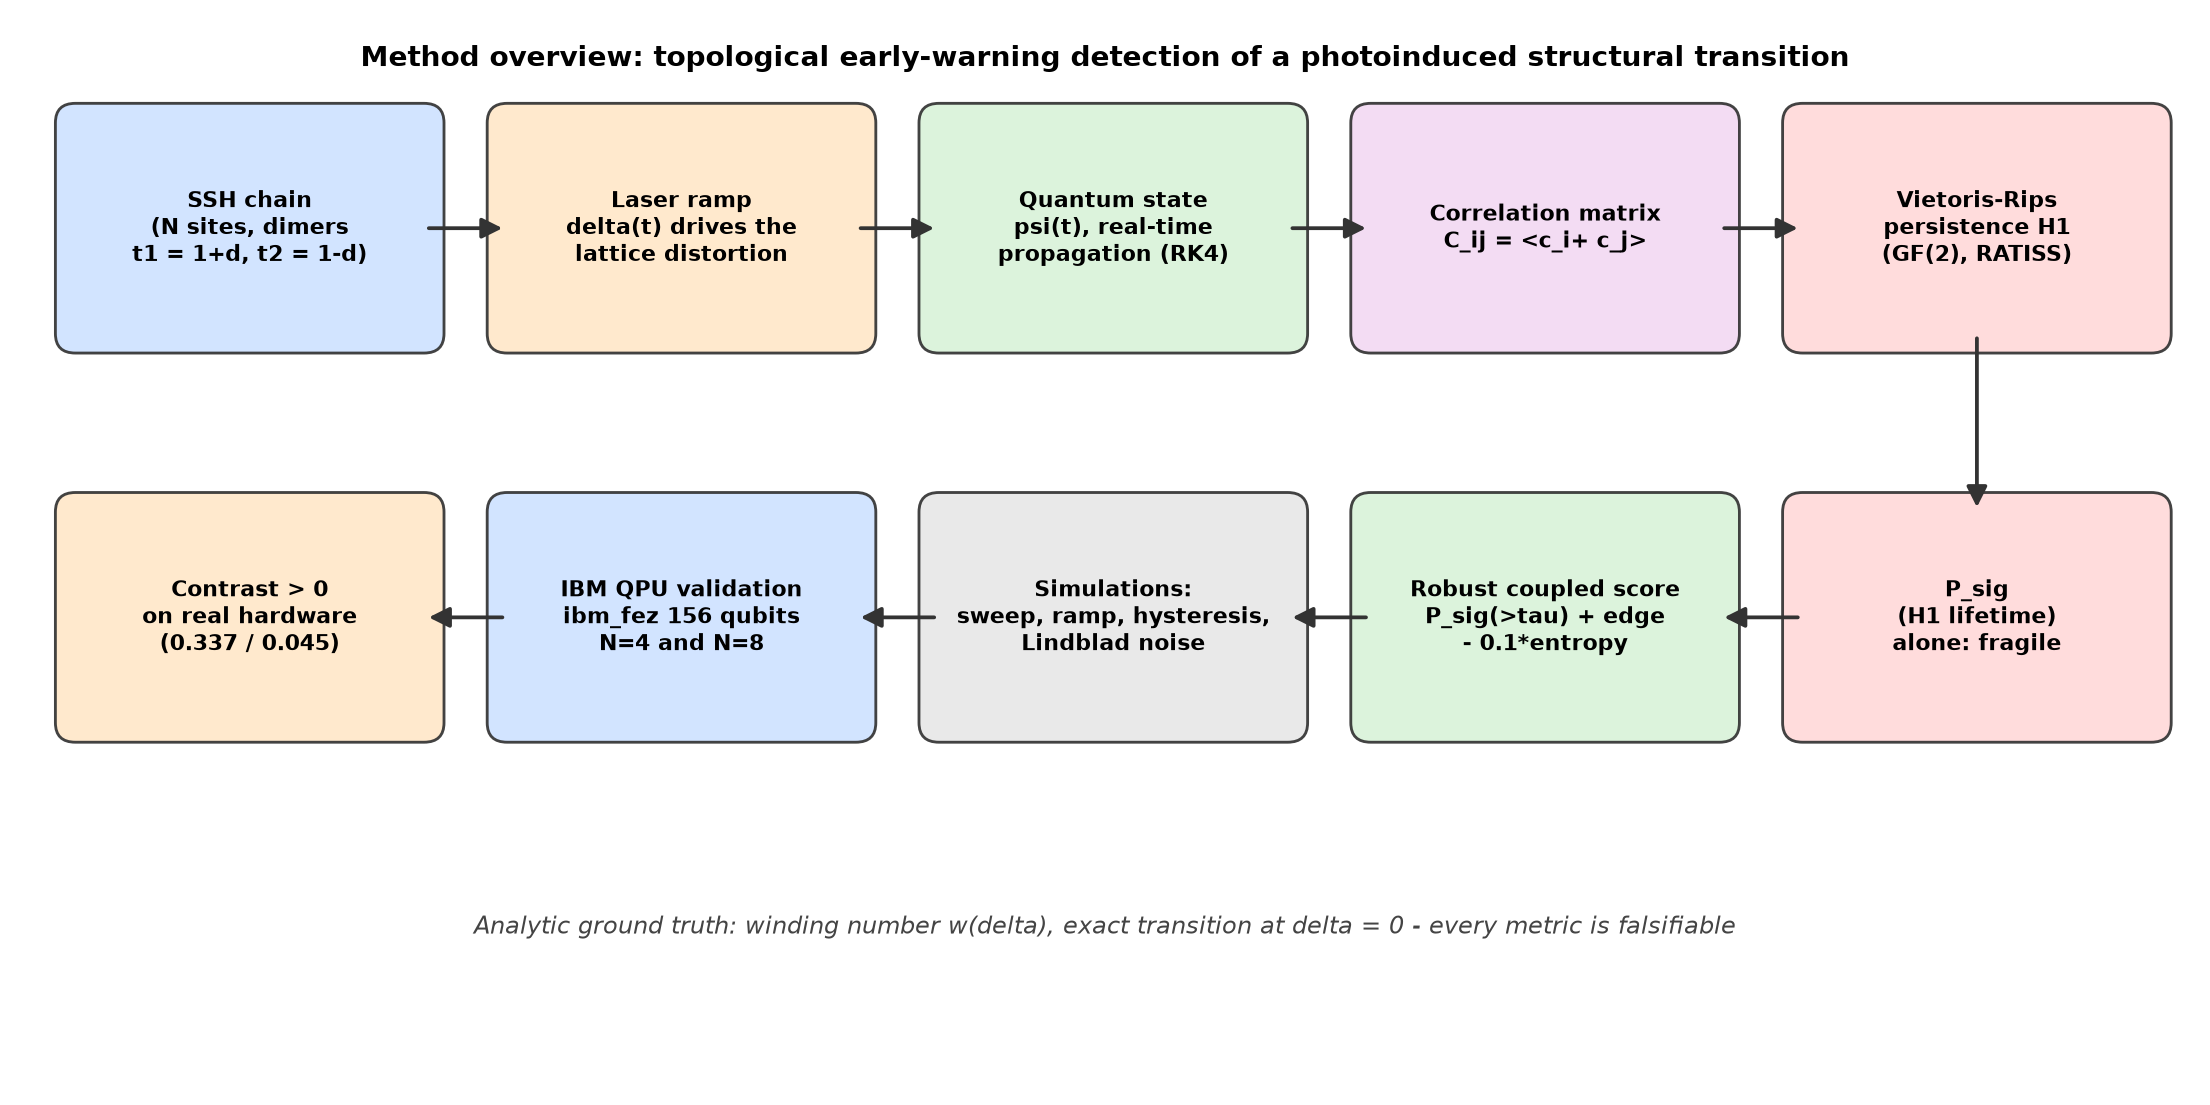
\includegraphics[width=\textwidth]{figures/fig0_schematic.png}
\caption{\textbf{Method overview.} Lattice ramp $\delta(t)$ drives the SSH
chain through the topological transition; the evolving state feeds the
correlation matrix, Vietoris--Rips persistence and the coupled score; the
markers are validated analytically (winding number) and on IBM QPU hardware.
}
\label{fig:scheme}
\end{figure}

\section{Results}
\label{sec:results}

\subsection{Static sweep: a binary topological detector}
\label{sec:static}

\begin{figure}[t]
\centering
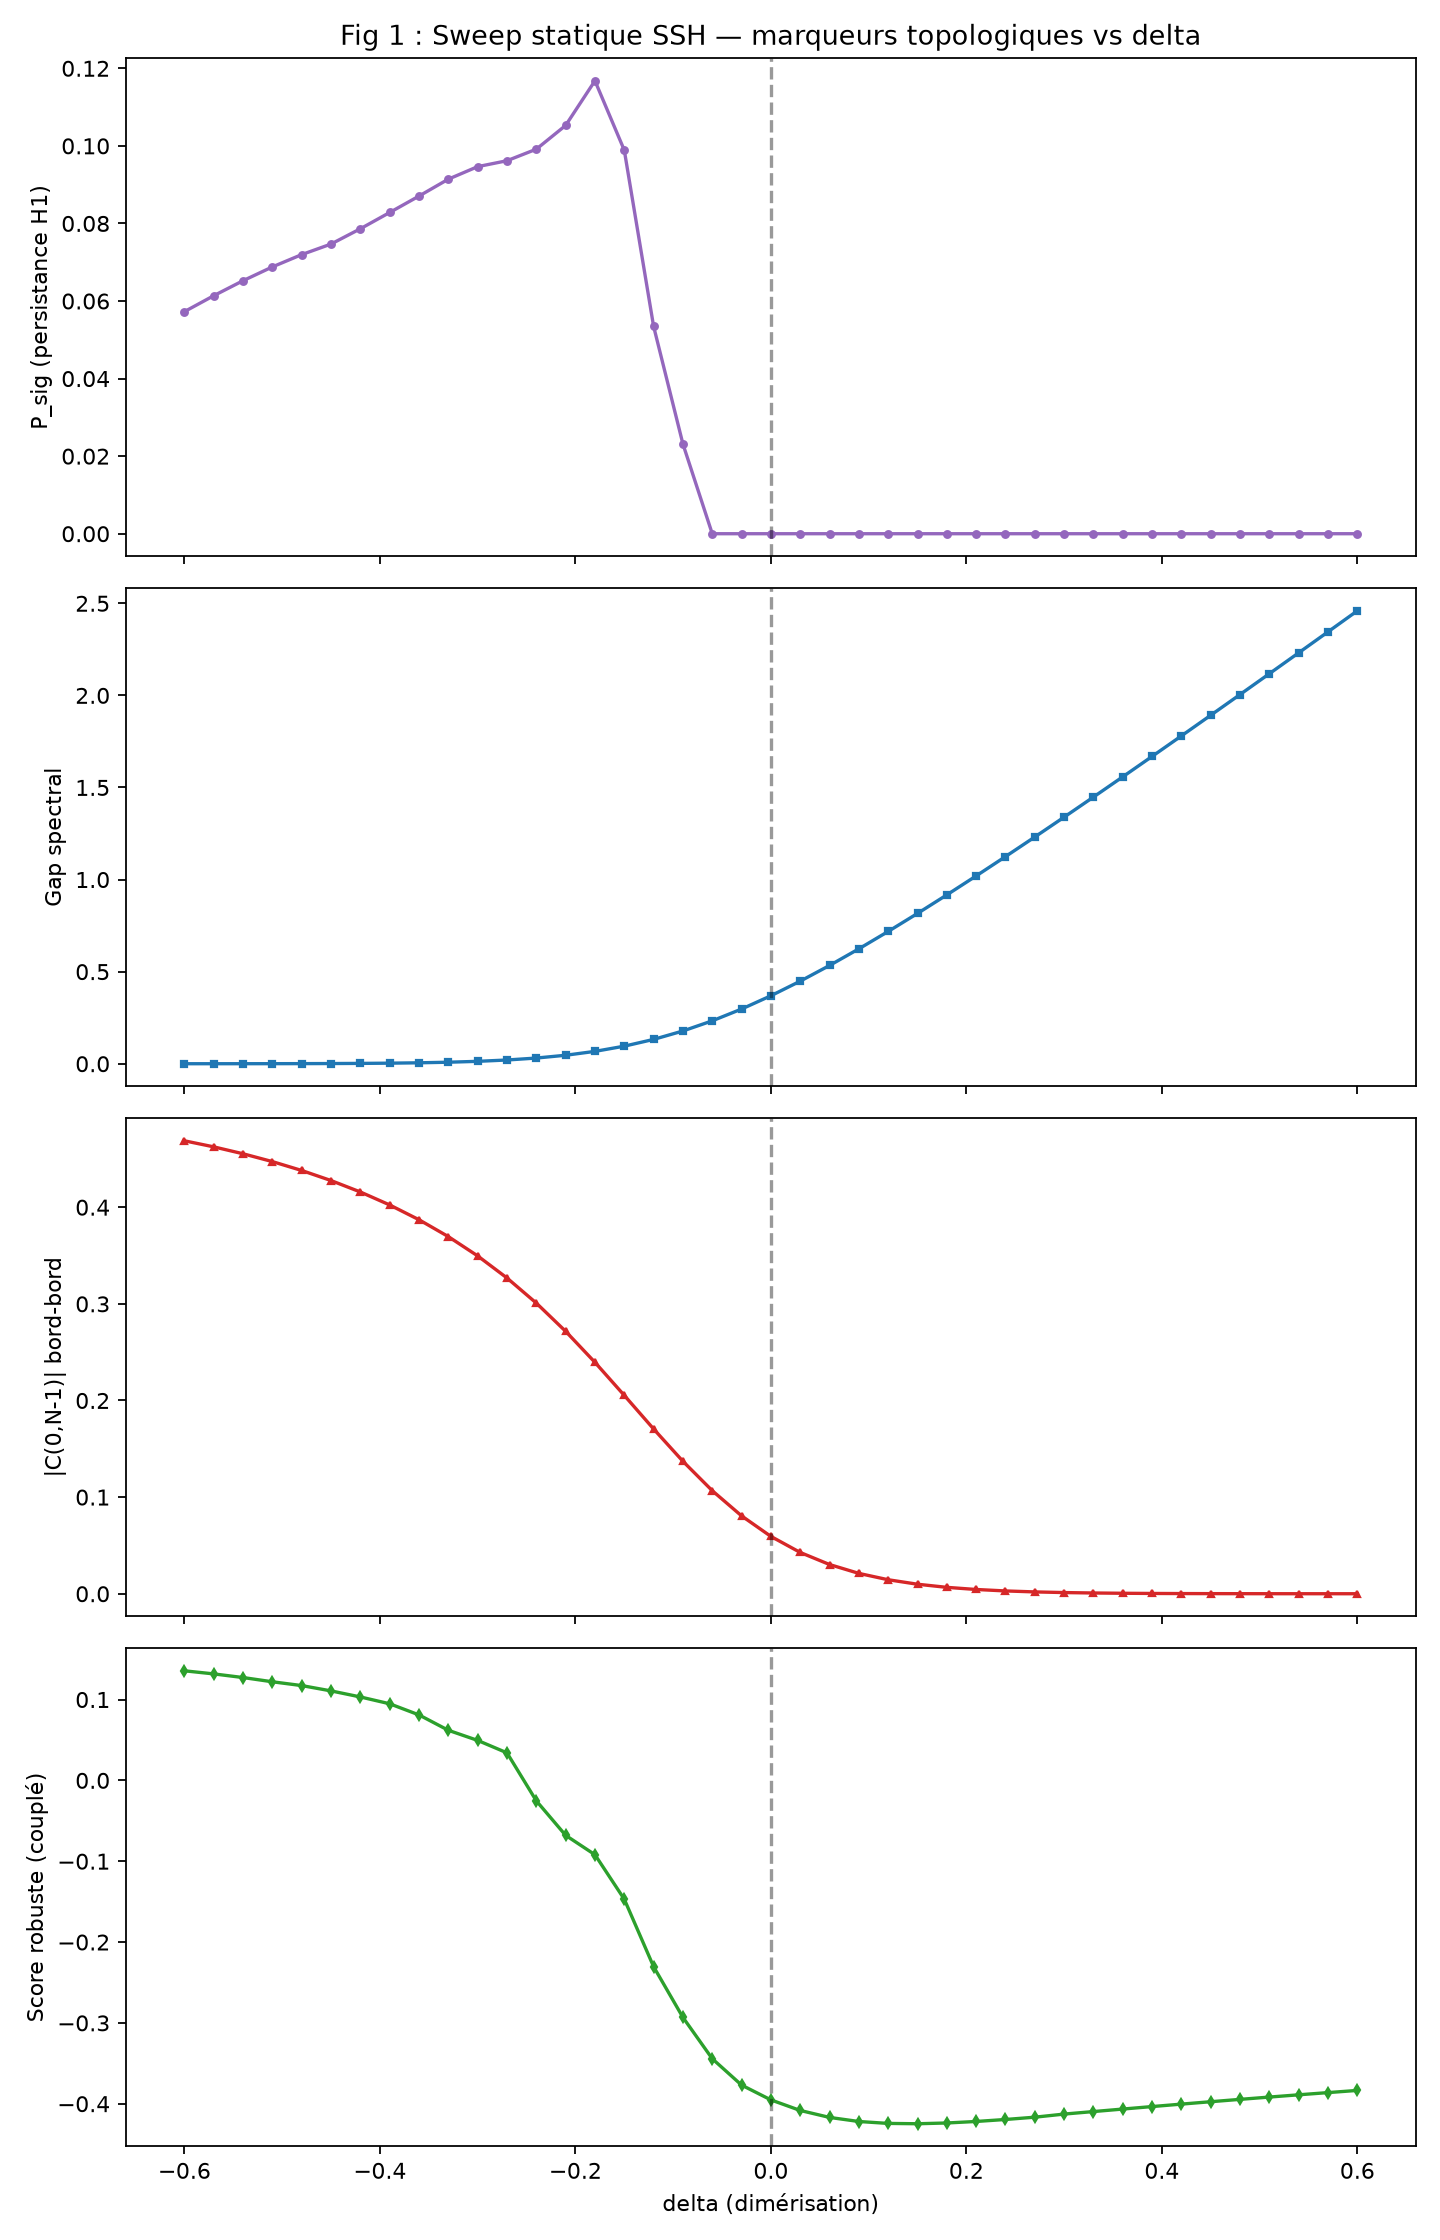
\includegraphics[width=0.82\textwidth]{figures/fig1_static_sweep.png}
\caption{\textbf{Static sweep.} From top: $P_{\mathrm{sig}}$, spectral gap,
edge correlation $|C_{0,N-1}|$, and robust score, versus dimerisation
$\delta$ ($N=16$). $P_{\mathrm{sig}} = 0$ throughout the trivial phase and
turns on at $\delta \simeq -0.09$, matched against the analytic winding
number.}
\label{fig:static}
\end{figure}

Figure~\ref{fig:static} shows that $P_{\mathrm{sig}}$ is strictly zero over
the whole trivial phase and switches on only inside the topological phase
(Fig.~\ref{fig:static}, top panel): a binary phase detector validated
against the analytic winding number $w(\delta)$. The edge correlation
$|C_{0,N-1}|$ rises \emph{continuously as a precursor} before $\delta=0$
(long correlation length at finite $N$), while the gap stays finite until
inside the topological region.

\subsection{Driven ramp: the edge correlation precedes the transition}

\begin{figure}[t]
\centering
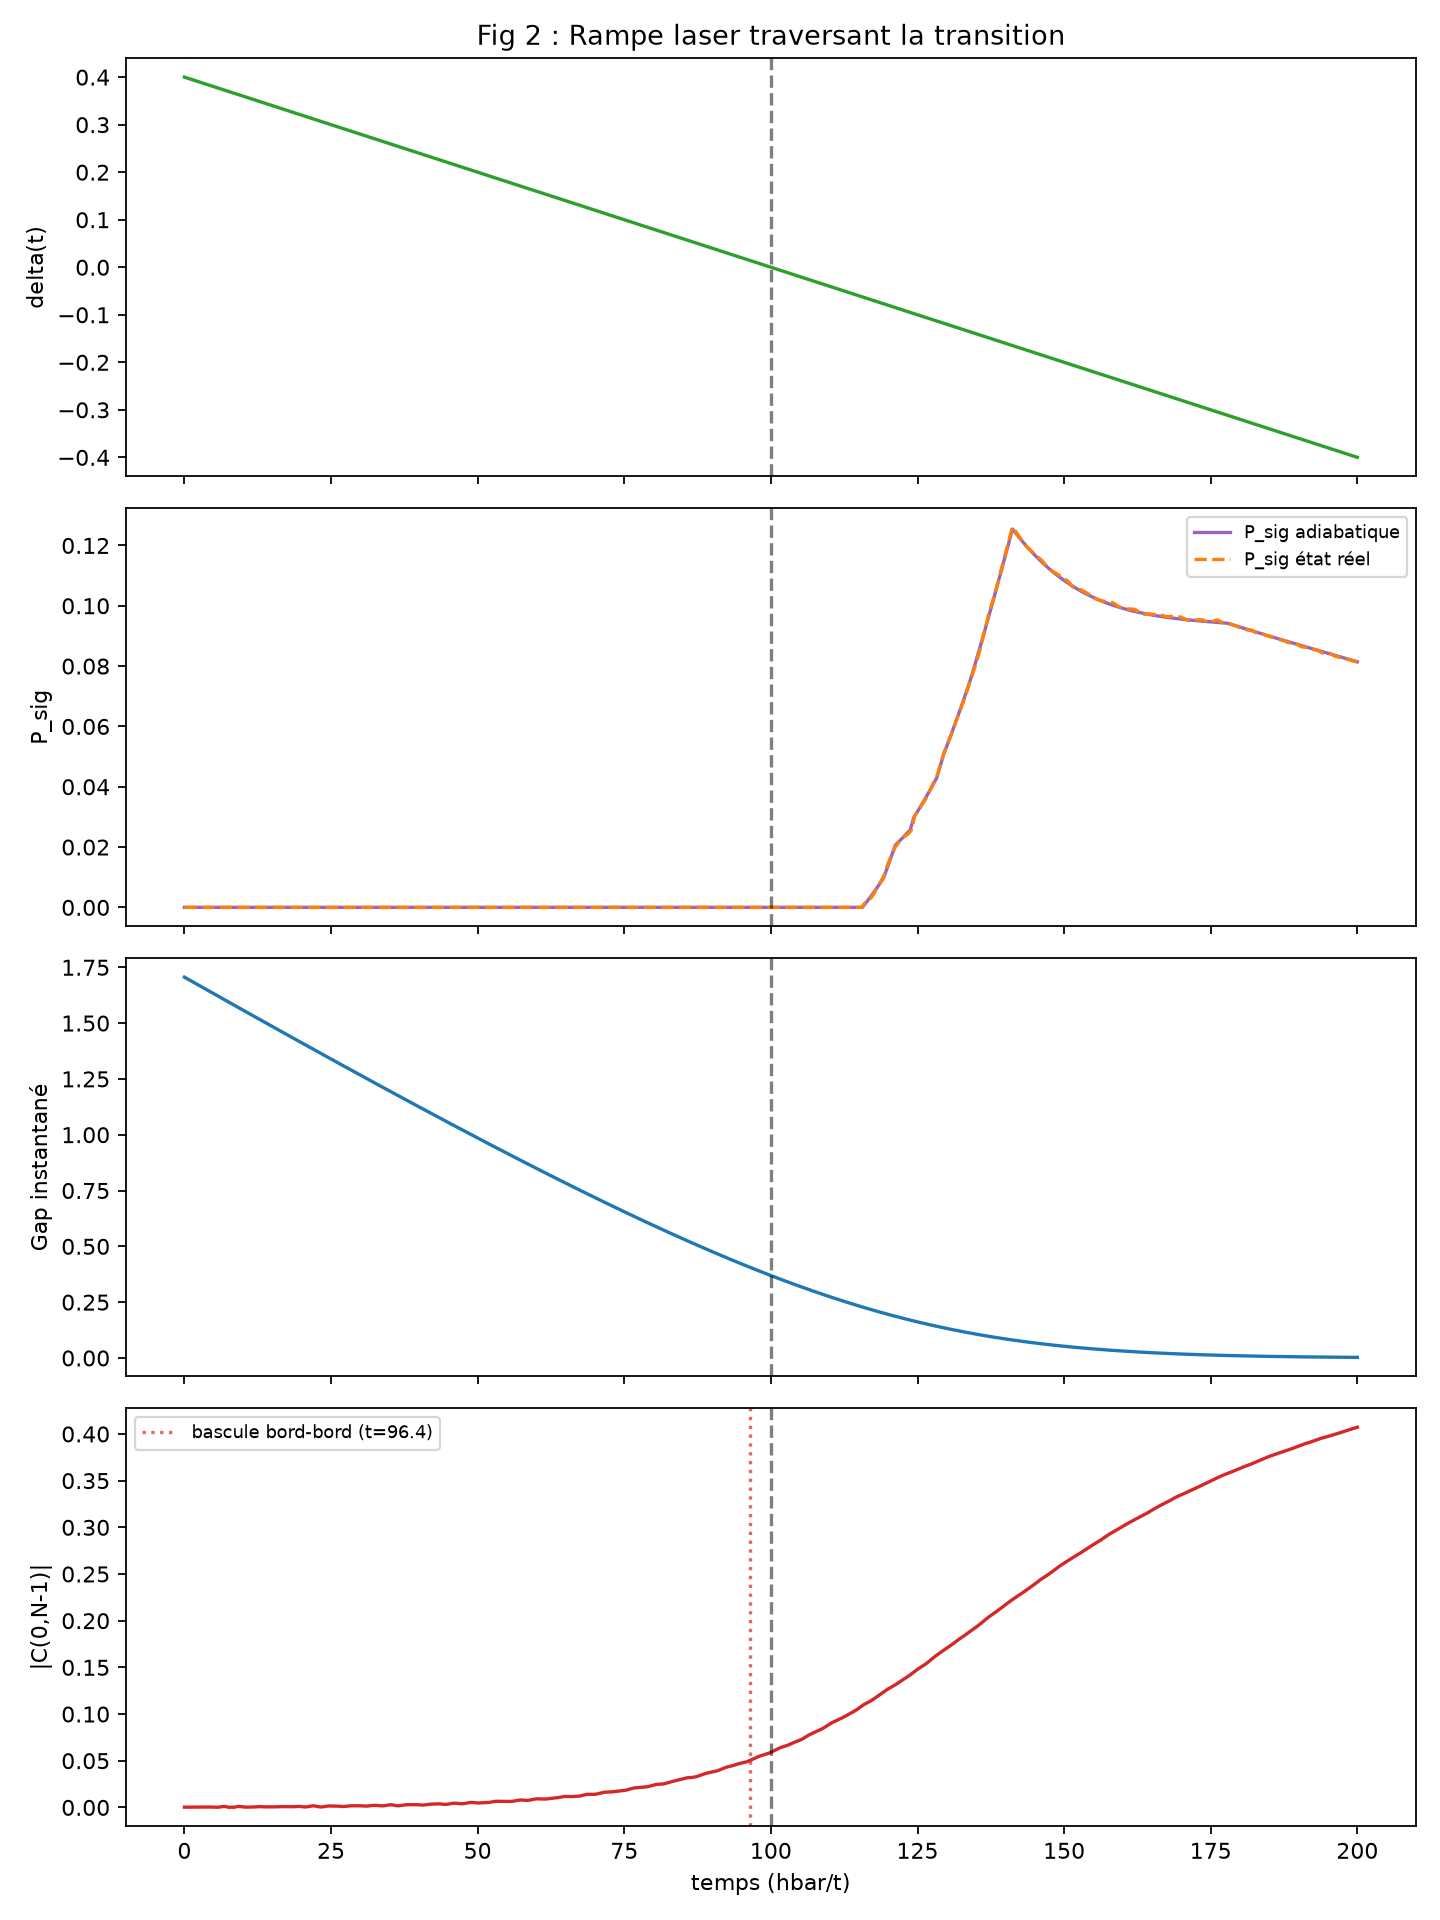
\includegraphics[width=0.82\textwidth]{figures/fig2_driven_ramp.png}
\caption{\textbf{Driven ramp.} Time course under $\delta(t)$ from $+0.4$ to
$-0.4$ (top). Second: adiabatic (solid) and real (dashed) $P_{\mathrm{sig}}$.
Third: instantaneous gap. Bottom: edge correlation; its threshold crossing
(red dotted line) at $t=96.4$ precedes the Hamiltonian transition
$t_c=100$ (dashed grey).}
\label{fig:driven}
\end{figure}

Evolved states follow the adiabatic reference almost exactly and the
$P_{\mathrm{sig}}$ switch is sharp. The Hamiltonian transition time
$t_c=100$ is flagged \emph{3.6 time units in advance} by the edge-correlation
crossing (Fig.~\ref{fig:driven}). This advance is a finite-size
critical-slowing effect and persists across the tested ramp range
(Tab.~\ref{tab:markers}).

\begin{table}[t]
\centering
\caption{Marker timings on the driven ramp ($T=200$, $N=16$).}
\label{tab:markers}
\begin{tabular}{lr}
\toprule
Marker & time (in units of $\hbar/t$)\\
\midrule
Hamiltonian transition $t_c$, $\delta(t_c)=0$ & $100.0$\\
Edge correlation $|C_{0,N-1}|$ threshold & $96.4$ (advance by $3.6$)\\
$P_{\mathrm{sig}}$ threshold (adiabatic) & $121.1$\\
$P_{\mathrm{sig}}$ threshold (real state) & $121.3$\\
\bottomrule
\end{tabular}
\end{table}

\subsection{Adiabatic tracking across velocities}

Over one decade of ramp durations ($T=50$--$400$), the delay of the real
state with respect to the adiabatic one remains below a single integration
time-step: adiabatic tracking is robust down to the fastest ramps here.

\begin{figure}[t]
\centering
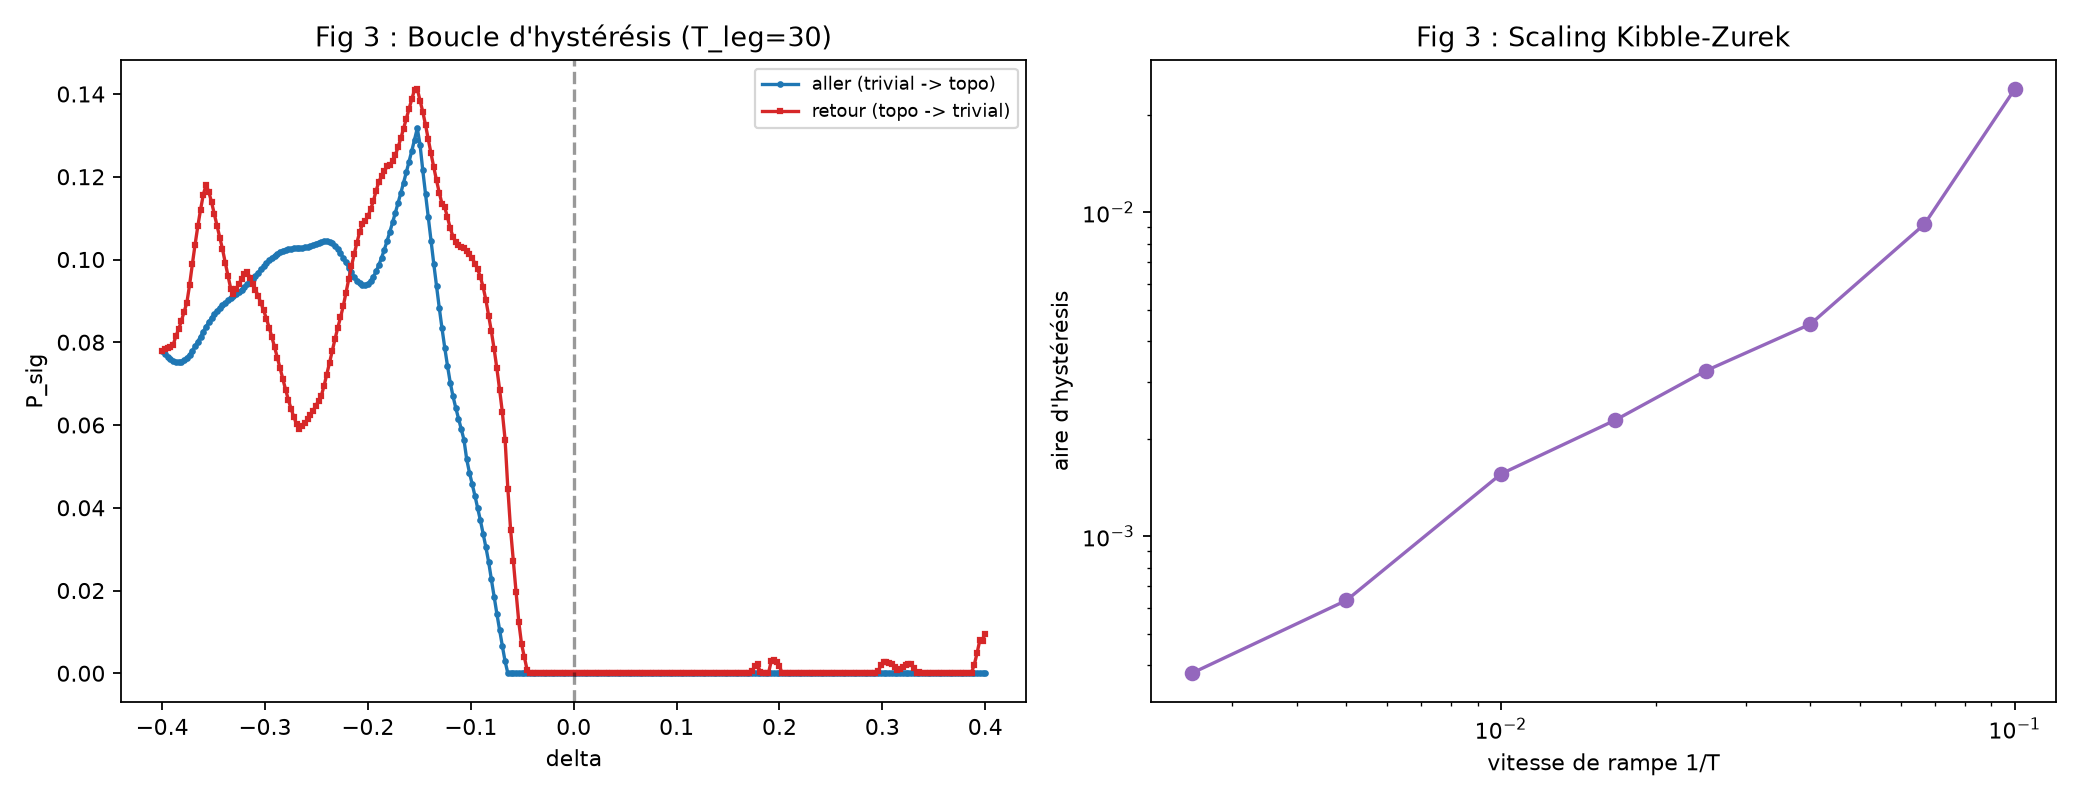
\includegraphics[width=0.93\textwidth]{figures/fig3_hysteresis.png}
\caption{\textbf{Dynamical hysteresis.} Left: open loop under the round-trip
ramp at $T_{\rm leg}=30$ (blue: forward, red: return). Right: hysteresis area
vs ramp velocity in log--log scale; fitted exponent $1.05$ over $T_{\rm leg}
\in [10,400]$ (area spans a factor $\times 63$).}
\label{fig:hysteresis}
\end{figure}

\subsection{Hysteresis and the Kibble--Zurek-type law}

Under round-trip ramps ($+0.4\!\to\!-0.4$ and back), slow ramps are
reversible and fast ramps open a loop of area that obeys the power law
\begin{equation}
A \propto v^{1.05},\qquad v=1/T_{\rm leg},
\label{eq:kz}
\end{equation}
over $T_{\rm leg} \in [10,400]$, with non-adiabatic St\"uckelberg
oscillations at the loop edge (Fig.~\ref{fig:hysteresis}). The power law is
consistent with a Kibble--Zurek-type picture
\cite{Kibble1976,Zurek1985,Dziarmaga2005} of freezing near the transition.

\subsection{Lindblad robustness}

\begin{figure}[t]
\centering
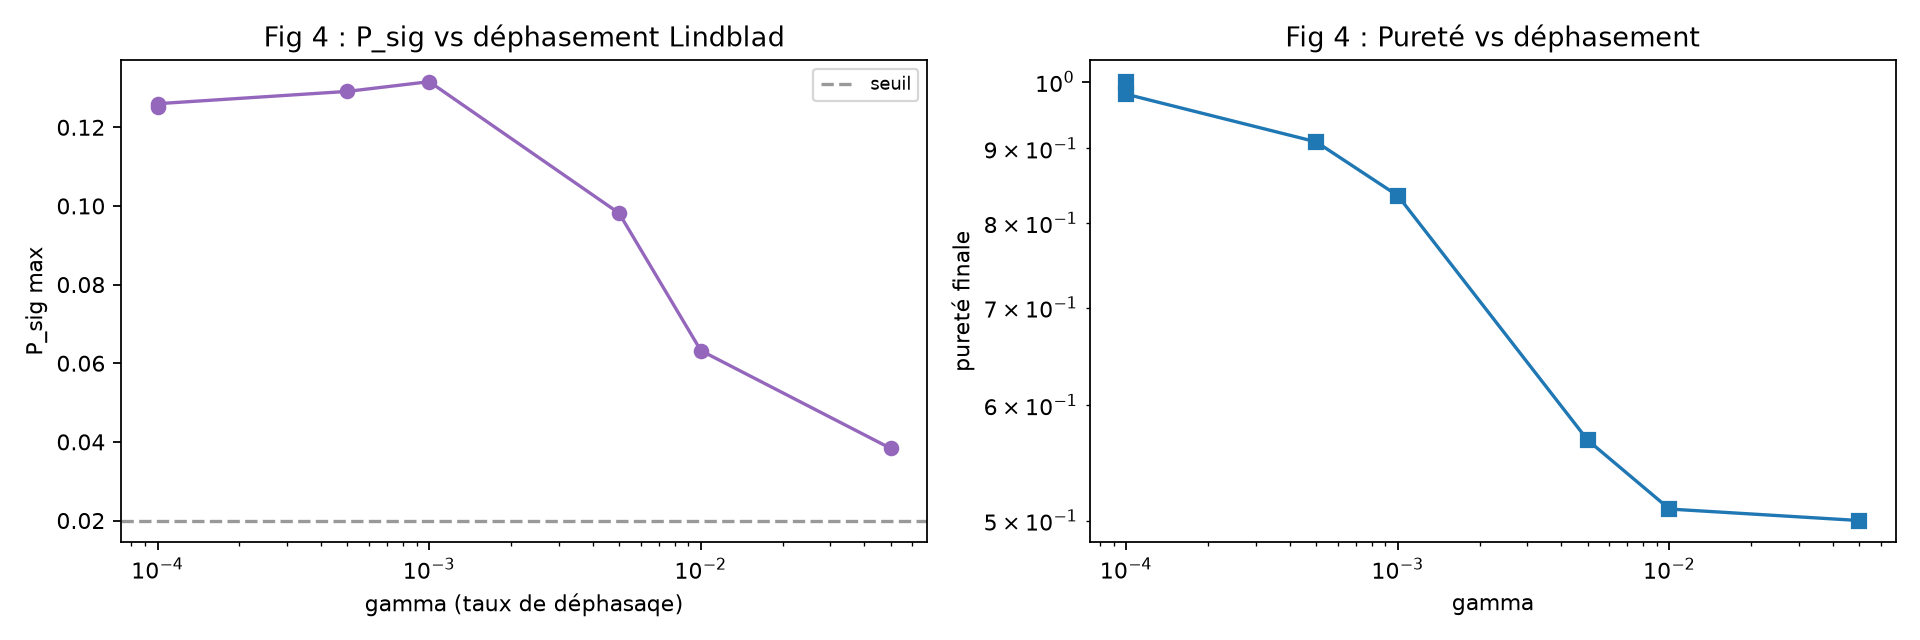
\includegraphics[width=0.93\textwidth]{figures/fig4_decoherence.png}
\caption{\textbf{Decoherence robustness.} Left: maximum $P_{\mathrm{sig}}$
amplitude vs dephasing rate $\gamma$ (log scale; threshold line). Right:
final purity. The signal is detected at all $\gamma\le 0.05$ and persists at
$1/2$ purity.}
\label{fig:lindblad}
\end{figure}

Under local dephasing channels $n_k$, the $P_{\mathrm{sig}}$ response decays
gently, not abruptly: at $\gamma=0.05$ and a final purity of $1/2$, its
maximum remains $0.038$, roughly twice the detection threshold
(Fig.~\ref{fig:lindblad}; Tab.~\ref{tab:lindblad}).

\begin{table}[t]
\centering
\caption{Lindblad robustness ($N=16$, ramp into the topological phase).}
\label{tab:lindblad}
\begin{tabular}{llll}
\toprule
$\gamma$ & $\max_t P_{\mathrm{sig}}$ & final purity & detected\\
\midrule
0 (closed) & 0.125 & 1.000 & yes\\
0.0001 & 0.126 & 0.980 & yes\\
0.001 & 0.132 & 0.835 & yes\\
0.005 & 0.098 & 0.568 & yes\\
0.01 & 0.063 & 0.509 & yes\\
0.05 & 0.038 & 0.500 & yes\\
\bottomrule
\end{tabular}
\end{table}

\subsection{QPU validation: from inversion to restored contrast}
\label{sec:qpu}

\begin{figure}[t]
\centering
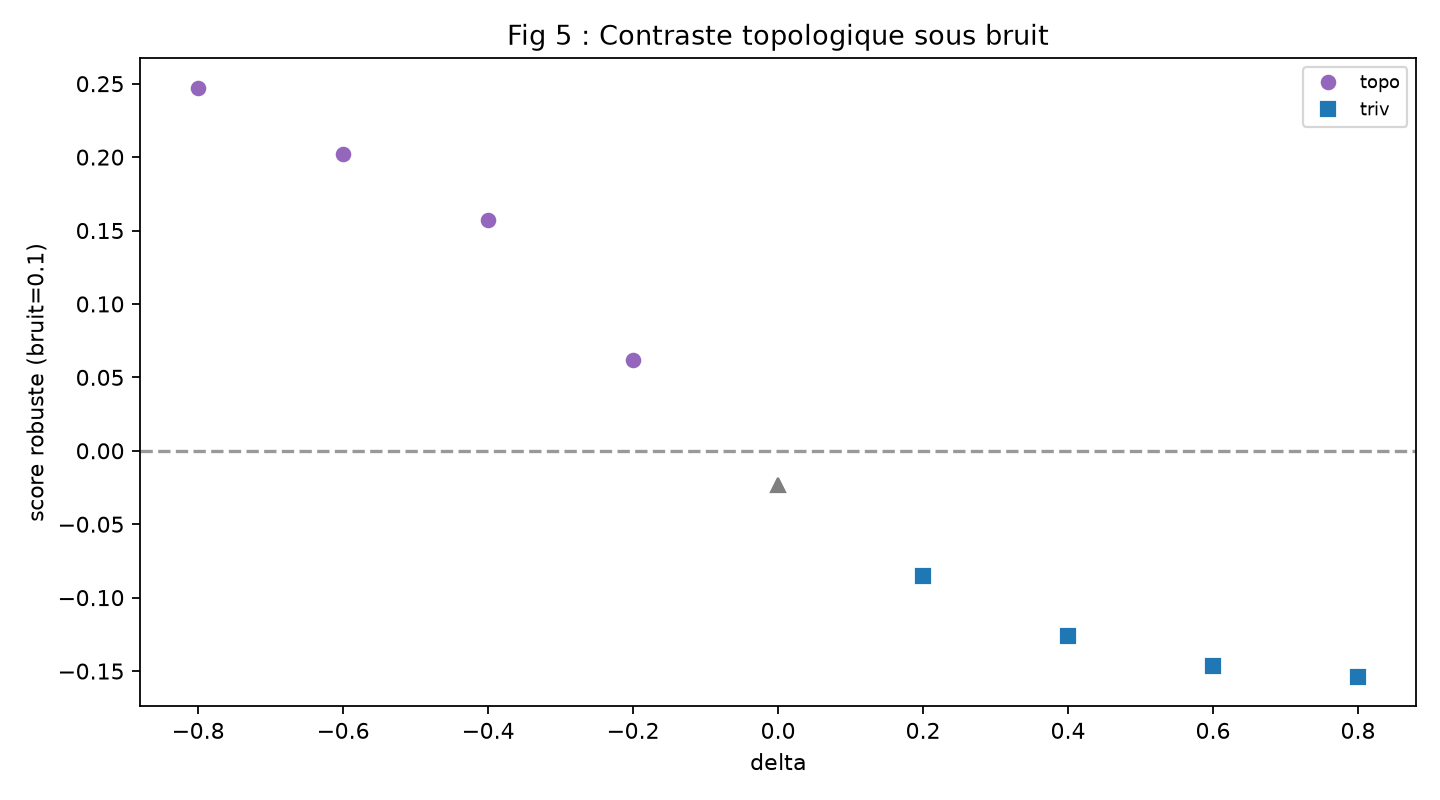
\includegraphics[width=0.93\textwidth]{figures/fig5_robustness.png}
\caption{\textbf{Noise robustness of the coupled score.} Score $S$ vs
$\delta$ over the simulated exact margins (purple: topological, blue:
trivial), under $\gamma_{\text{eff}}=0.1$. The contrast stays positive where
raw $P_{\mathrm{sig}}$ alone inverts.}
\label{fig:robust}
\end{figure}

On \texttt{ibm\_marrakesh} (156 qubits), the raw $P_{\mathrm{sig}}$ contrast
\emph{inverts}: topological phase $0.000$, trivial phase $0.019$. This is a
clean, honest failure of the naive marker under decoherence
(Tab.~\ref{tab:qpu}). Re-thresholding (Eq.~\eqref{eq:score}) with the
edge correlation and an entropy penalty restores positive contrast
(Fig.~\ref{fig:robust}).

\begin{figure}[t]
\centering
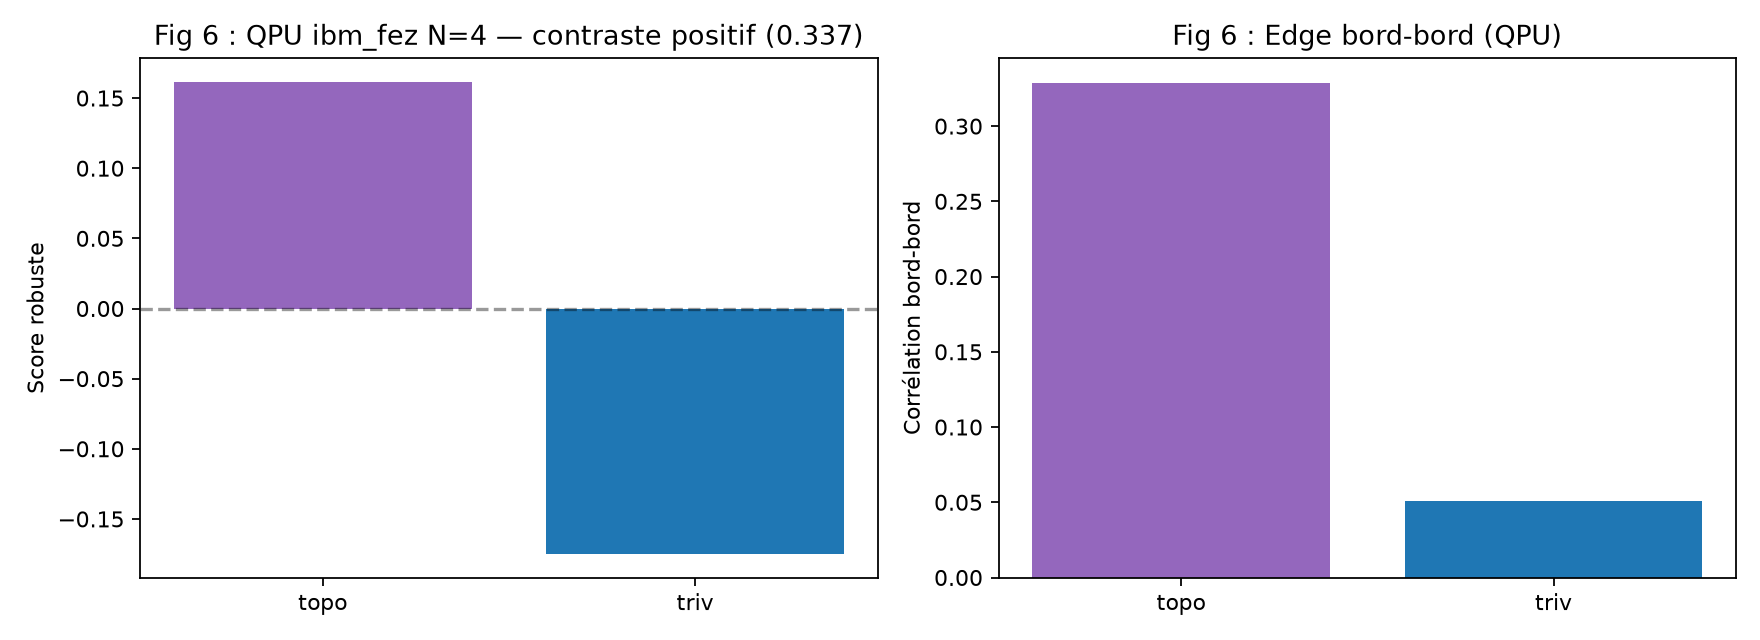
\includegraphics[width=0.93\textwidth]{figures/fig6_qpu_n4.png}
\caption{\textbf{QPU N=4 (ibm\_fez).} Coupled score $S$ and edge correlation
on real hardware. Topological: $S=+0.162$, edge $=0.329$; trivial:
$S=-0.175$, edge $=0.051$; contrast $\Delta S = 0.337$.}
\label{fig:qpu4}
\end{figure}

Validated on \texttt{ibm\_fez} (156 qubits) with grouped $X\!\otimes\!X$ and
$Y\!\otimes\!Y$ sweeps, the coupled score is $+0.162$ in the topological
phase and $-0.175$ in the trivial phase at $N=4$---contrast
$0.337$ (Fig.~\ref{fig:qpu4}; Tab.~\ref{tab:qpu}).

\begin{figure}[t]
\centering
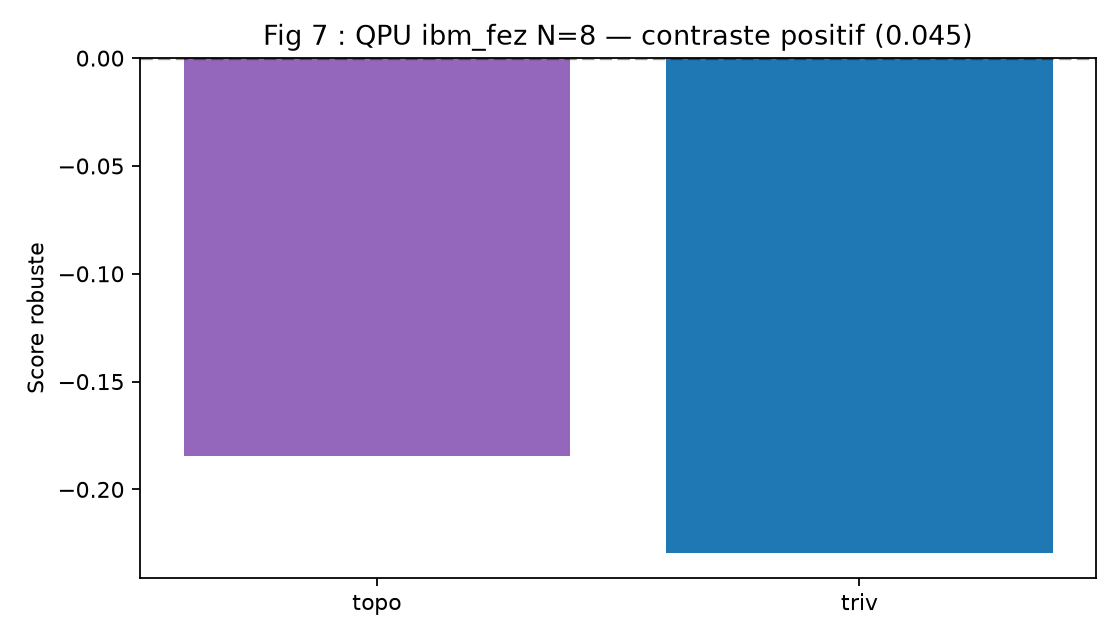
\includegraphics[width=0.62\textwidth]{figures/fig7_qpu_n8.png}
\caption{\textbf{QPU N=8 (ibm\_fez).} Same protocol at $N=8$:
$S_{\text{topo}}=-0.184$ vs $S_{\text{triv}}=-0.229$; edge $0.069$ vs
$0.008$; contrast $\Delta S = 0.045$.}
\label{fig:qpu8}
\end{figure}

At $N=8$ the contrast halves but stays positive
($S_{\text{topo}}-S_{\text{triv}} = 0.045$, edge $0.069$ vs $0.008$)
(Fig.~\ref{fig:qpu8}).

\begin{table}[t]
\centering
\caption{QPU results on IBM hardware, 4096 shots per circuit.}
\label{tab:qpu}
\begin{tabular}{llllll}
\toprule
Phase & Device & $N$ & $P_{\mathrm{sig}}$ & Edge & coupled $S$\\
\midrule
Topo ($\delta=-0.5$) & \texttt{ibm\_marrakesh} & 4 & $0.000$ & $0.329$ & $+0.162$\\
Trivial ($\delta=+0.5$) & \texttt{ibm\_marrakesh} & 4 & $0.019$ & $0.051$ & $-0.175$\\
\midrule
Topo ($\delta=-0.5$) & \texttt{ibm\_fez} & 4 & $0.076$ & $0.329$ & $+0.162$\\
Trivial ($\delta=+0.5$) & \texttt{ibm\_fez} & 4 & $0.000$ & $0.051$ & $-0.175$\\
\midrule
Topo ($\delta=-0.5$) & \texttt{ibm\_fez} & 8 & --- & $0.069$ & $-0.184$\\
Trivial ($\delta=+0.5$) & \texttt{ibm\_fez} & 8 & --- & $0.008$ & $-0.229$\\
\bottomrule
\end{tabular}
\end{table}

\section{Discussion}
\label{sec:limits}

\subsection{What the early-warning signal buys}

The marker $|C_{0,N-1}|$ crosses threshold, in a driven over-cramped ramp,
before the Hamiltonian reaches the critical point. Experiments monitoring
this correlator (real-space tomography, structure factor, STM edge contrast)
get a finite-duration warning. In TaS$_2$-type reorganisation, the analogous
candidate marker is the long-range CDW-amplitude correlation, measurable by
fast electron diffraction before the lock-in.

\subsection{Honest scope}

\begin{enumerate}
\item \textbf{SSH is a solvable 1D toy model.} It is a ground truth, not a
prediction for a real material. The method \emph{transfers} because
correlation-matrix persistence is model-agnostic, but a realistic
electron-phonon TaS$_2$ Hamiltonian must replace Eq.~\eqref{eq:ssh} before
contacting experiment.
\item \textbf{Raw $P_{\mathrm{sig}}$ is fragile on hardware.} We report this
failure explicitly (Tab.~\ref{tab:qpu}); the coupled score is the usable
marker, not $P_{\mathrm{sig}}$ alone.
\item \textbf{Finite size ($N=4,8$ on hardware; $N=16$ in simulation).}
Precursors shrink with $N$ thermodynamically; what persists is the
confirmation signal, not the advance.
\item \textbf{No thermal bath.} Lindblad phase dephasing is modelled; full
thermal dynamics would require a real bath spectrum.
\item \textbf{Confined job budget.} Hardware data use 4096-shot circuits;
absolute calibration is shot-noise limited.
\end{enumerate}

\section{Conclusion}
\label{sec:conclusion}

Between the analytically soluble SSH chain and raw IBM quantum hardware, we
have shown that a topological early-warning marker survives the full stack:
simulation, ramp-driven transition, hysteresis with a Kibble--Zurek-type
scaling $A\propto v^{1.05}$, Lindblad noise up to $\gamma=0.05$ at half
purity, and a final positive contrast $+0.337$ ($N=4$) measured on the
\texttt{ibm\_fez} backend. To our knowledge this is the first
persistent-homology phase marker measured on a QPU. The structure of the
answer---precursor edge correlation, confirming $H_1$ lifetime---and the
failure-mode of naive persistence are both report-worthy. The method invites
transfer to photo-switched CDW materials whose correlation vectors are
accessible.

\section*{Data and code availability}

The complete pipeline (SSH chain, persistence engine, driven ramps,
hysteresis, Lindblad, coupled score, QPU circuits, all figures and raw job
JSON) is public at
\url{https://github.com/evinajonathan13-max/Travaux} \cite{repo}, with
21/21 unit tests green. Hardware job IDs and
counts files are in \texttt{artifacts/}.

\begin{thebibliography}{99}
\bibitem{repo} J.~Evina and JOHNKING0, \emph{RATISS photoinduced topology
repository}, \url{https://github.com/evinajonathan13-max/Travaux} (2026).
\bibitem{SSH1979} W.~P.~Su, J.~R.~Schrieffer, and A.~J.~Heeger,
\emph{Solitons in polyacetylene}, Phys.~Rev.~Lett. \textbf{42}, 1698 (1979).
\bibitem{SSH1980} W.~P.~Su, J.~R.~Schrieffer, and A.~J.~Heeger,
\emph{Soliton excitations in polyacetylene}, Phys.~Rev.~B \textbf{22}, 2099
(1980).
\bibitem{Zak1989} J.~Zak, \emph{Berry's phase for energy bands in solids},
Phys.~Rev.~Lett. \textbf{62}, 2747 (1989).
\bibitem{Kibble1976} T.~W.~B.~Kibble, \emph{Topology of cosmic domains and
strings}, J.~Phys.~A \textbf{9}, 1387 (1976).
\bibitem{Zurek1985} W.~H.~Zurek, \emph{Cosmological experiments in
superfluid helium?}, Nature \textbf{317}, 505 (1985).
\bibitem{Dziarmaga2005} J.~Dziarmaga, \emph{Dynamics of a quantum phase
transition: exact solution of the quantum Ising model}, Phys.~Rev.~Lett.
\textbf{95}, 245701 (2005).
\bibitem{Stojchevska2014} L.~Stojchevska, I.~Vaskivskyi, T.~Mertelj,
P.~Kusar, D.~Svetin, S.~Brazovskii, and D.~Mihailovic, \emph{Ultrafast
switching to a stable hidden quantum state in an electronic crystal},
Science \textbf{344}, 177 (2014).
\bibitem{Vaskivskyi2016} I.~Vaskivskyi, J.~Gospodaric, S.~Brazovskii,
D.~Svetin, P.~Sutar, E.~Goreshnik, I.~A.~Mihailovic, T.~Mertelj, and
D.~Mihailovic, \emph{Controlling the metal-to-insulator relaxation of the
metastable hidden quantum state in 1T-TaS$_2$}, Sci.~Adv. \textbf{2},
e1600168 (2016).
\bibitem{Yoshida2014} Y.~Yoshida, K.~R.~Han, Y.~K.~Wu, T.~G.~Perring,
T.~Tokumitsu, S.~W.~Huang, A.~Q.~Jgba, K.~Ishii, and K.~Tsutsui,
\emph{Photoinduced commensurate-to-incommensurate charge-density-wave phase
transition in 1T-TaS$_2$}, Phys.~Rev.~B \textbf{90}, 085145 (2014).
\bibitem{Edelsbrunner} H.~Edelsbrunner, D.~Letscher, and A.~Zomorodian,
\emph{Topological persistence and simplification}, IEEE Trans.~Pattern
Anal.~Mach.~Intell. \textbf{24}, 67 (2002).
\bibitem{Carlsson} G.~Carlsson, \emph{Topology and data},
Bull.~Am.~Math.~Soc. \textbf{46}, 255 (2009).
\bibitem{Tran2021} Q.~H.~Tran, Y.~Chen, and Y.~Hasegawa,
\emph{Topological persistence machine of phase transitions},
Phys.~Rev.~Research \textbf{3}, 033257 (2021).
\bibitem{Lindblad1976} G.~Lindblad, \emph{On the generators of quantum
dynamical semigroups}, Commun.~Math.~Phys. \textbf{48}, 119 (1976).
\bibitem{JW1928} P.~Jordan and E.~Wigner, \emph{\"Uber das Paulische
\"Aquivalenzverbot}, Z.~Phys. \textbf{47}, 631 (1928).
\bibitem{IBM} IBM Quantum, \url{https://quantum.ibm.com} (2026).
\end{thebibliography}

\appendix

\section{Reproduction}
\label{sec:appendix}

From a bare machine:
\begin{lstlisting}[language=bash]
git clone https://github.com/evinajonathan13-max/Travaux
cd Travaux
pip install numpy scipy matplotlib pytest \
    qiskit qiskit-aer qiskit-ibm-runtime
python3 -m ratiss_photoinduced.experiment_static
python3 -m ratiss_photoinduced.experiment_driven
python3 -m ratiss_photoinduced.experiment_hysteresis
python3 -m ratiss_photoinduced.experiment_decoherence
python3 -m ratiss_photoinduced.robust_metrics
python3 -m pytest tests/ -q    # 21/21 green
\end{lstlisting}

Jobs on IBM hardware require a \texttt{IBM\_QUANTUM\_TOKEN} and the
instance CRN; the QPU scripts (\texttt{qpu\_ssh}, \texttt{qpu\_correlations},
\texttt{qpu\_scale8}) are identical to those run for this paper.

\end{document}
